\SourceLeaf{310}
\begin{center}
\textbf{\Large NACHLASS UND BRIEFWECHSEL.}\par\bigskip
\textbf{[DAS DREIECK.]}
\end{center}
\bigskip

Die Aufgabe, die Lage eines Punktes aus dem bekannten Verhältniss seiner Abstände von dreien der Lage nach bekannten Punkten zu finden.

Coordinaten der gegebenen Punkte $\left\{\begin{array}{c}a,a',a''\\b,b',b''\end{array}\right\}$; des unbekannten $\left\{\begin{array}{c}x\\y\end{array}\right\}$; Verhältniss der drei Abstände wie $m$, $m'$, $m''$.

\textls{Erste Auflösungsart.}

Man mache
\[
\begin{array}{lll}
a''-a'=h\cos A,&a-a''=h'\cos A',&a'-a=h''\cos A''\\
b''-b'=h\sin A,&b-b''=h'\sin A',&b'-b=h''\sin A''
\end{array}
\]
\noindent und nehme an
\[
\begin{aligned}
x&=a+r\cos\varphi\\
y&=b+r\sin\varphi.
\end{aligned}
\]

So hat man die Gleichungen:
\[
\begin{aligned}
rr-2rh''\cos(\varphi-A'')+h''h''&=\frac{rrm'm'}{mm}\\
rr+2rh'\cos(\varphi-A')+h'h'&=\frac{rrm''m''}{mm}.
\end{aligned}
\]
\begin{center}\resizebox{4.4cm}{!}{%
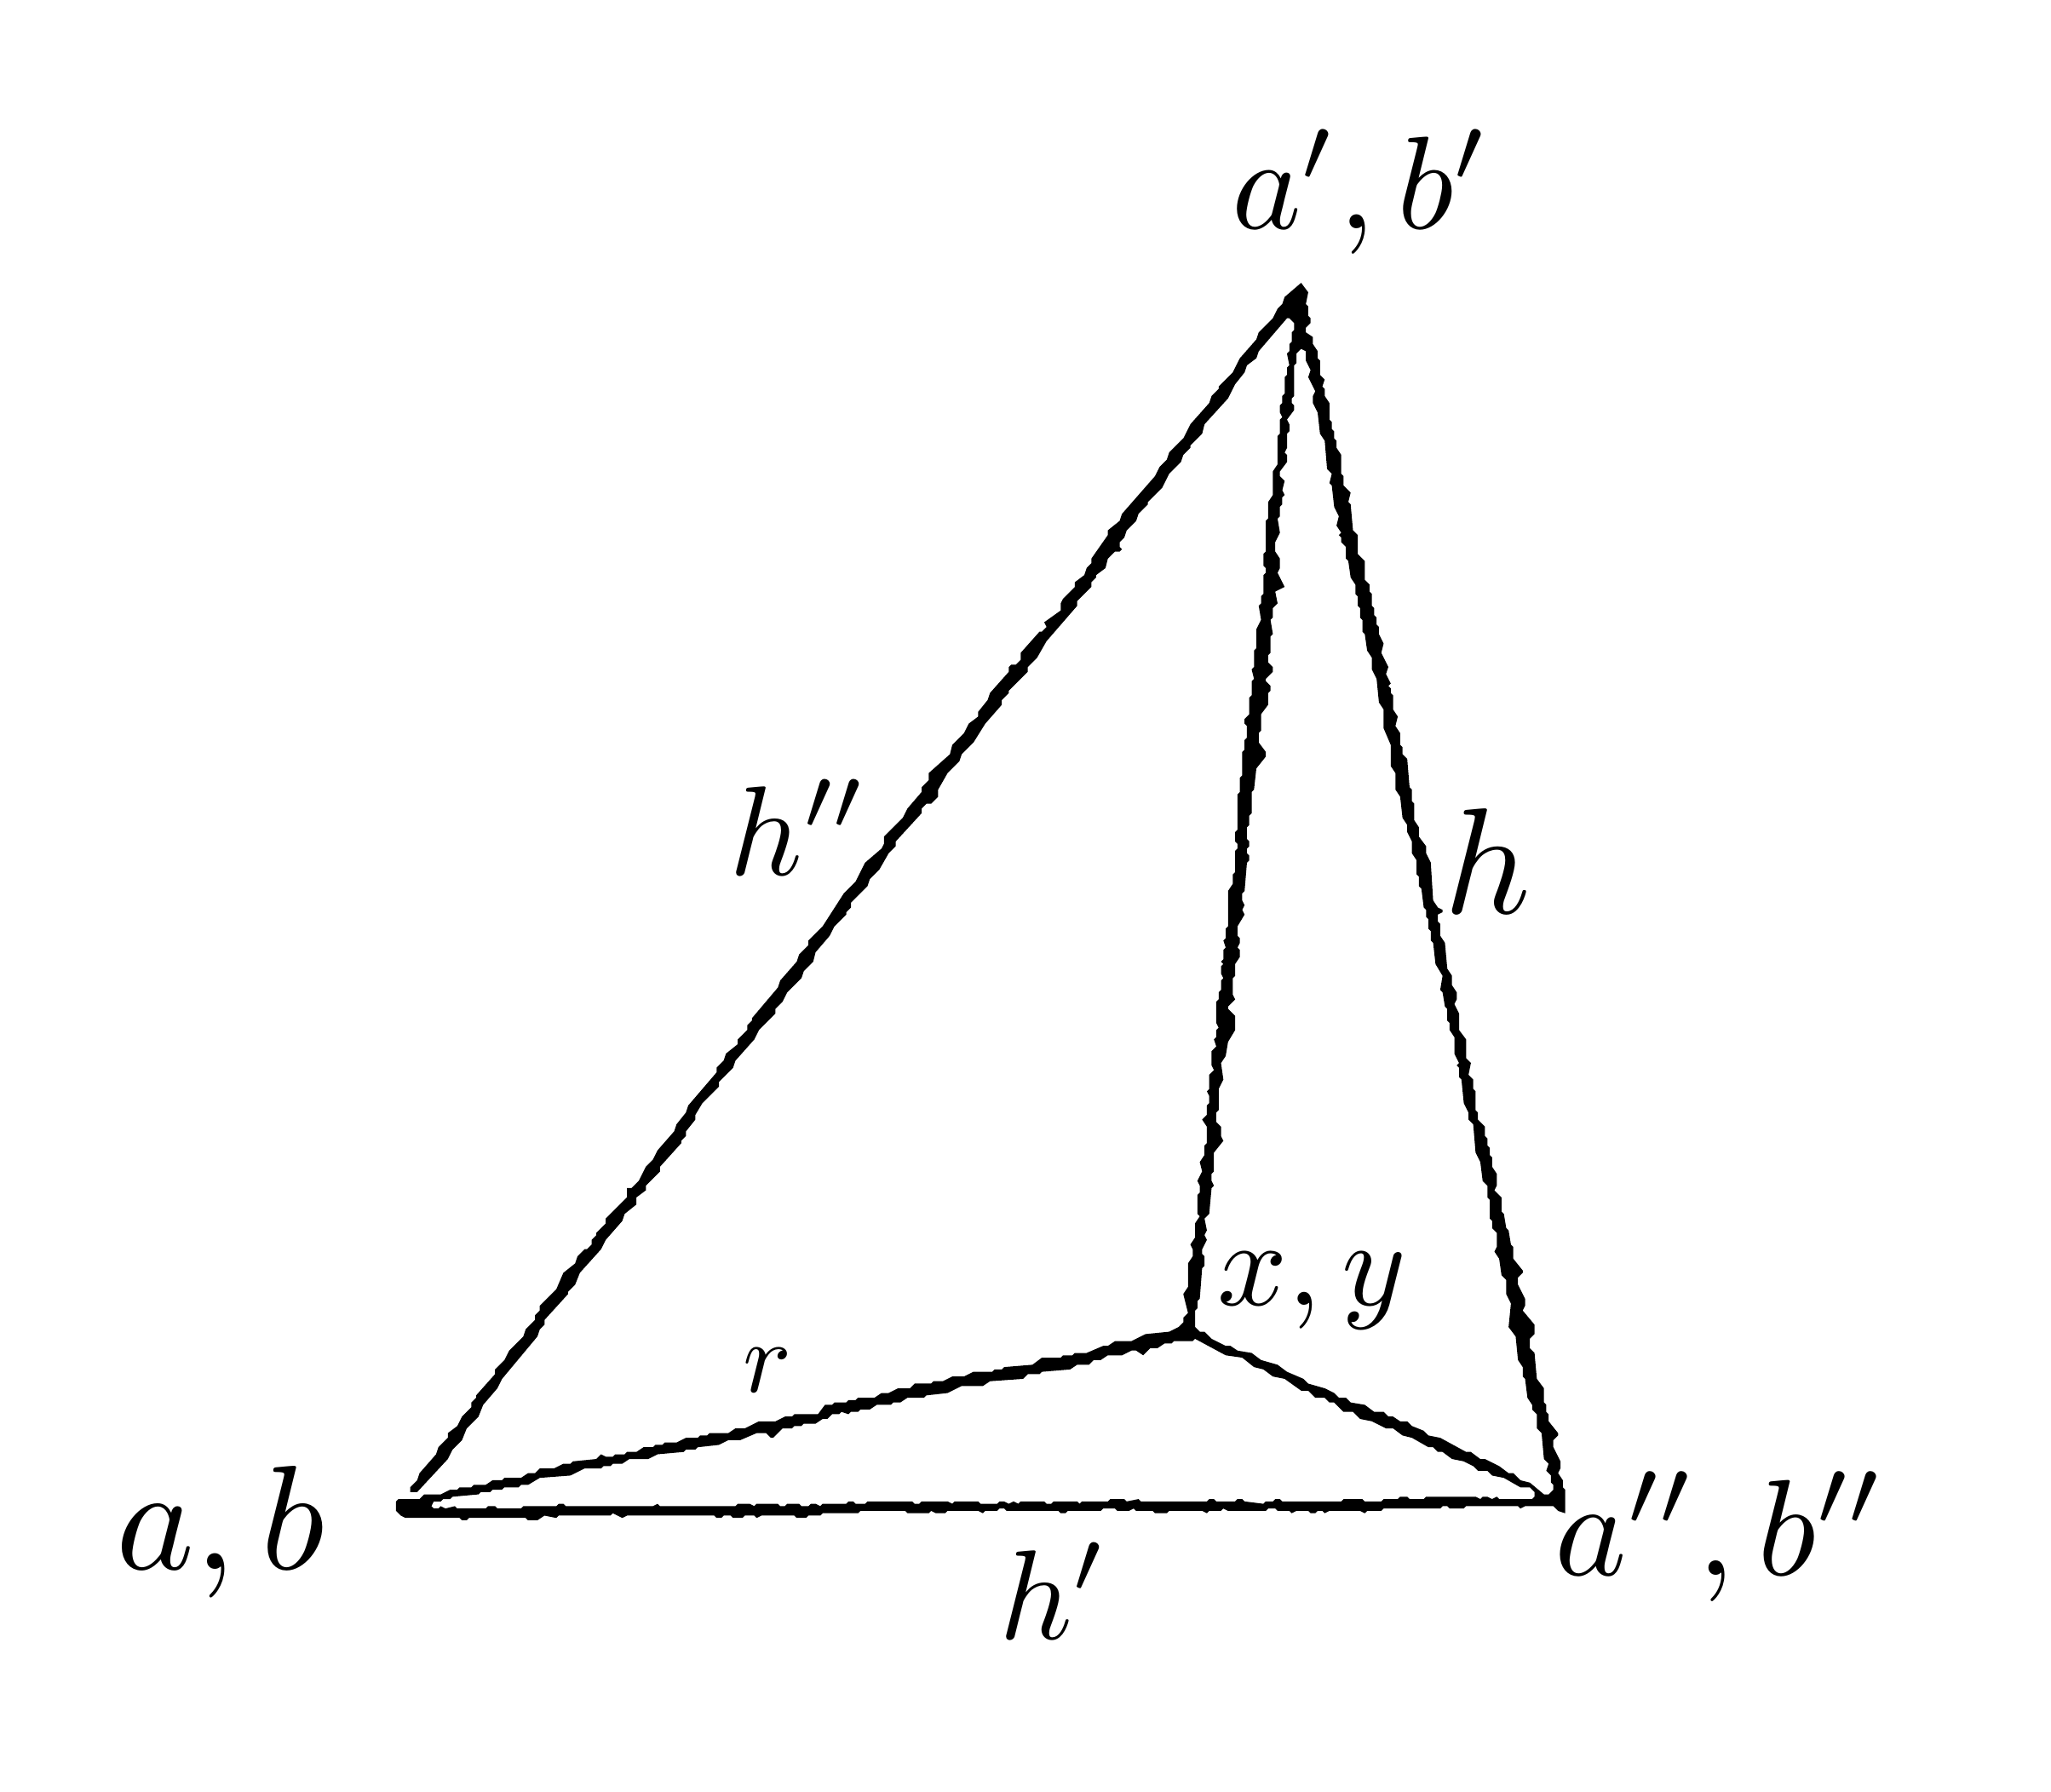
\begin{tikzpicture}[x=1pt,y=-1pt]
\path[use as bounding box] (0,0) rectangle (850,740);
\path[fill=black,draw=none,even odd rule]
(542,110) -- (535,116) -- (534,119) -- (532,121) -- (530,125) -- (524,131) -- (523,134) -- (516,142) -- (513,148) -- (507,154) -- (507,155) -- (504,158) -- (503,161) -- (495,170) -- (492,176) -- (486,182) -- (485,185) -- (482,188) -- (480,192) -- (466,208) -- (465,211) -- (460,215) -- (460,217) -- (453,227) -- (453,229) -- (451,231) -- (450,234) -- (446,237) -- (446,239) -- (441,244) -- (440,246) -- (440,249) -- (433,254) -- (434,256) -- (432,258) -- (431,258) -- (423,267) -- (423,270) -- (421,272) -- (419,272) -- (418,273) -- (418,275) -- (410,284) -- (409,287) -- (405,292) -- (405,294) -- (401,297) -- (399,301) -- (394,306) -- (393,310) -- (384,318) -- (384,321) -- (381,324) -- (381,326) -- (375,333) -- (373,337) -- (365,345) -- (365,348) -- (364,350) -- (357,356) -- (353,364) -- (348,369) -- (339,383) -- (333,389) -- (333,391) -- (329,395) -- (328,398) -- (321,406) -- (320,409) -- (309,422) -- (309,423) -- (307,425) -- (307,427) -- (303,431) -- (303,433) -- (298,437) -- (297,440) -- (294,443) -- (294,445) -- (282,459) -- (281,462) -- (277,467) -- (276,470) -- (269,478) -- (267,482) -- (264,485) -- (261,491) -- (258,494) -- (256,494) -- (256,498) -- (247,507) -- (247,509) -- (243,513) -- (243,514) -- (241,516) -- (241,518) -- (239,520) -- (238,520) -- (235,523) -- (234,526) -- (229,530) -- (226,537) -- (219,544) -- (219,546) -- (217,548) -- (217,550) -- (213,554) -- (212,557) -- (206,563) -- (204,567) -- (200,571) -- (200,573) -- (192,582) -- (192,583) -- (190,585) -- (190,587) -- (186,591) -- (184,595) -- (180,598) -- (180,600) -- (176,604) -- (175,607) -- (168,615) -- (167,618) -- (164,621) -- (164,623) -- (167,623) -- (180,609) -- (182,605) -- (186,601) -- (188,596) -- (193,591) -- (195,586) -- (201,579) -- (203,575) -- (218,557) -- (219,554) -- (221,552) -- (221,550) -- (231,539) -- (231,538) -- (234,535) -- (236,530) -- (245,520) -- (247,516) -- (254,508) -- (255,505) -- (260,501) -- (260,498) -- (264,495) -- (264,493) -- (270,487) -- (270,485) -- (279,475) -- (279,474) -- (281,472) -- (281,470) -- (285,465) -- (285,463) -- (288,458) -- (295,451) -- (295,449) -- (301,443) -- (302,440) -- (310,431) -- (312,427) -- (319,420) -- (319,418) -- (322,415) -- (324,411) -- (330,405) -- (331,402) -- (335,398) -- (336,394) -- (342,387) -- (344,383) -- (349,378) -- (349,377) -- (351,375) -- (351,373) -- (358,366) -- (359,363) -- (363,359) -- (367,352) -- (370,349) -- (370,347) -- (381,335) -- (381,333) -- (383,331) -- (385,331) -- (388,328) -- (388,325) -- (392,318) -- (397,313) -- (398,310) -- (403,305) -- (408,297) -- (415,289) -- (415,287) -- (418,284) -- (418,283) -- (426,275) -- (426,273) -- (430,269) -- (434,262) -- (447,247) -- (447,245) -- (453,239) -- (453,237) -- (455,235) -- (455,234) -- (459,231) -- (460,227) -- (463,224) -- (465,224) -- (466,223) -- (465,222) -- (465,220) -- (467,218) -- (468,215) -- (472,211) -- (473,208) -- (477,204) -- (477,203) -- (483,197) -- (486,191) -- (491,186) -- (492,183) -- (495,180) -- (495,179) -- (500,174) -- (501,170) -- (511,159) -- (514,153) -- (518,148) -- (519,145) -- (523,142) -- (524,139) -- (536,125) -- (537,125) -- (539,127) -- (539,130) -- (538,131) -- (538,135) -- (537,136) -- (537,139) -- (536,140) -- (537,145) -- (536,146) -- (536,149) -- (535,150) -- (535,157) -- (534,158) -- (534,161) -- (533,162) -- (533,165) -- (534,167) -- (533,168) -- (533,174) -- (532,175) -- (532,187) -- (530,190) -- (530,200) -- (528,203) -- (528,210) -- (527,211) -- (527,224) -- (526,225) -- (526,230) -- (527,231) -- (527,233) -- (526,234) -- (526,242) -- (525,243) -- (525,246) -- (524,247) -- (525,253) -- (523,257) -- (523,265) -- (522,266) -- (522,273) -- (521,274) -- (522,278) -- (521,279) -- (521,285) -- (520,286) -- (520,293) -- (518,295) -- (518,297) -- (519,298) -- (519,303) -- (518,304) -- (518,308) -- (517,309) -- (517,319) -- (516,320) -- (516,326) -- (515,327) -- (515,342) -- (514,343) -- (514,347) -- (515,348) -- (515,350) -- (514,351) -- (514,360) -- (513,361) -- (513,365) -- (511,368) -- (511,383) -- (510,384) -- (510,388) -- (509,389) -- (510,392) -- (509,393) -- (509,397) -- (508,398) -- (509,399) -- (508,400) -- (508,403) -- (509,405) -- (508,406) -- (508,410) -- (507,411) -- (507,414) -- (506,415) -- (506,424) -- (507,426) -- (506,427) -- (506,430) -- (505,431) -- (506,434) -- (504,436) -- (504,442) -- (505,444) -- (503,446) -- (503,452) -- (502,453) -- (503,455) -- (503,458) -- (502,459) -- (502,463) -- (500,465) -- (502,468) -- (502,475) -- (501,476) -- (501,480) -- (499,483) -- (500,487) -- (498,491) -- (499,493) -- (499,496) -- (498,497) -- (498,505) -- (499,506) -- (497,509) -- (497,515) -- (495,518) -- (496,520) -- (496,523) -- (494,526) -- (494,536) -- (492,539) -- (494,547) -- (492,549) -- (492,551) -- (490,553) -- (486,555) -- (476,556) -- (470,559) -- (463,559) -- (460,561) -- (458,561) -- (451,564) -- (446,564) -- (445,565) -- (441,565) -- (440,566) -- (432,566) -- (428,569) -- (416,570) -- (415,571) -- (412,571) -- (411,572) -- (403,572) -- (399,574) -- (394,574) -- (390,576) -- (386,576) -- (385,577) -- (378,577) -- (376,579) -- (371,579) -- (367,581) -- (364,581) -- (361,583) -- (354,583) -- (353,584) -- (350,584) -- (349,585) -- (344,585) -- (343,586) -- (340,586) -- (337,590) -- (327,590) -- (326,591) -- (323,591) -- (319,593) -- (312,593) -- (306,596) -- (302,596) -- (299,598) -- (291,598) -- (290,599) -- (287,599) -- (286,600) -- (281,600) -- (277,602) -- (272,602) -- (271,603) -- (268,603) -- (267,604) -- (263,604) -- (260,606) -- (256,606) -- (255,607) -- (251,607) -- (250,608) -- (247,608) -- (245,607) -- (243,609) -- (233,610) -- (232,611) -- (229,611) -- (225,613) -- (219,613) -- (217,615) -- (214,615) -- (211,617) -- (204,617) -- (203,618) -- (199,618) -- (196,620) -- (191,620) -- (190,621) -- (185,621) -- (184,622) -- (181,622) -- (177,624) -- (170,624) -- (168,626) -- (159,626) -- (158,627) -- (158,631) -- (160,633) -- (162,634) -- (185,634) -- (186,635) -- (188,635) -- (189,634) -- (213,634) -- (214,635) -- (218,635) -- (221,633) -- (226,634) -- (227,633) -- (249,633) -- (250,632) -- (254,634) -- (256,633) -- (293,633) -- (294,634) -- (296,634) -- (297,633) -- (300,633) -- (301,634) -- (305,634) -- (306,633) -- (310,633) -- (311,634) -- (313,633) -- (327,633) -- (328,634) -- (332,634) -- (333,633) -- (338,633) -- (339,632) -- (354,632) -- (355,631) -- (374,631) -- (375,632) -- (384,632) -- (385,631) -- (387,632) -- (391,632) -- (392,631) -- (405,631) -- (407,632) -- (408,631) -- (413,631) -- (414,630) -- (416,630) -- (417,631) -- (439,631) -- (440,632) -- (442,632) -- (443,631) -- (457,631) -- (458,630) -- (463,630) -- (464,631) -- (469,631) -- (471,630) -- (472,631) -- (479,631) -- (480,632) -- (485,632) -- (486,631) -- (500,631) -- (502,632) -- (503,631) -- (508,631) -- (509,630) -- (511,631) -- (527,631) -- (528,630) -- (531,630) -- (532,631) -- (537,631) -- (538,632) -- (540,631) -- (545,631) -- (546,632) -- (548,632) -- (549,631) -- (551,631) -- (552,632) -- (554,631) -- (567,631) -- (569,632) -- (570,631) -- (576,631) -- (577,630) -- (601,630) -- (602,629) -- (604,629) -- (605,630) -- (611,630) -- (612,629) -- (634,629) -- (635,630) -- (637,629) -- (649,629) -- (651,631) -- (654,632) -- (654,622) -- (653,621) -- (653,618) -- (651,615) -- (652,613) -- (652,610) -- (649,604) -- (649,601) -- (651,599) -- (651,598) -- (647,593) -- (647,590) -- (646,589) -- (646,586) -- (645,585) -- (645,579) -- (642,575) -- (641,564) -- (639,562) -- (639,558) -- (641,556) -- (641,552) -- (636,546) -- (637,544) -- (637,541) -- (634,535) -- (634,532) -- (636,530) -- (636,529) -- (632,524) -- (632,519) -- (631,518) -- (630,512) -- (629,511) -- (628,505) -- (627,504) -- (627,498) -- (624,495) -- (625,493) -- (625,488) -- (623,485) -- (623,481) -- (622,480) -- (622,477) -- (621,476) -- (621,473) -- (620,472) -- (620,468) -- (617,465) -- (617,462) -- (616,461) -- (616,453) -- (615,452) -- (615,448) -- (613,446) -- (614,441) -- (612,439) -- (612,431) -- (609,427) -- (609,420) -- (607,416) -- (608,414) -- (608,411) -- (606,408) -- (606,404) -- (604,401) -- (603,390) -- (601,387) -- (601,382) -- (600,381) -- (600,378) -- (602,377) -- (602,376) -- (600,375) -- (598,372) -- (597,356) -- (595,352) -- (595,349) -- (592,345) -- (592,341) -- (590,338) -- (590,331) -- (589,330) -- (589,325) -- (588,324) -- (587,312) -- (585,310) -- (585,307) -- (584,306) -- (584,301) -- (582,298) -- (583,294) -- (581,291) -- (581,285) -- (580,284) -- (580,282) -- (579,281) -- (580,280) -- (578,276) -- (579,273) -- (576,267) -- (577,263) -- (575,259) -- (575,256) -- (574,255) -- (574,252) -- (573,251) -- (573,248) -- (572,247) -- (572,242) -- (571,241) -- (571,238) -- (569,236) -- (569,228) -- (566,225) -- (566,217) -- (564,215) -- (563,204) -- (562,203) -- (563,199) -- (560,196) -- (560,192) -- (559,191) -- (559,183) -- (557,180) -- (557,177) -- (556,176) -- (556,173) -- (555,172) -- (555,169) -- (554,168) -- (554,161) -- (552,158) -- (552,155) -- (551,154) -- (552,151) -- (550,149) -- (550,143) -- (549,142) -- (549,139) -- (547,136) -- (547,133) -- (544,131) -- (544,129) -- (546,127) -- (546,125) -- (545,124) -- (545,120) -- (544,119) -- (545,114) -- cycle
(641,623) -- (641,625) -- (640,626) -- (626,626) -- (625,625) -- (623,626) -- (621,625) -- (619,625) -- (618,626) -- (616,625) -- (595,625) -- (594,626) -- (588,626) -- (587,625) -- (584,625) -- (583,626) -- (577,626) -- (576,627) -- (569,627) -- (568,626) -- (560,626) -- (559,627) -- (534,627) -- (533,626) -- (531,626) -- (530,627) -- (527,627) -- (526,628) -- (518,627) -- (517,626) -- (515,626) -- (514,627) -- (506,627) -- (505,626) -- (503,626) -- (502,627) -- (474,627) -- (473,626) -- (468,627) -- (467,626) -- (461,626) -- (460,627) -- (449,627) -- (448,628) -- (447,627) -- (437,627) -- (436,628) -- (434,628) -- (433,627) -- (423,627) -- (422,628) -- (420,627) -- (418,628) -- (416,627) -- (414,627) -- (413,628) -- (406,628) -- (405,627) -- (395,627) -- (394,628) -- (392,627) -- (381,627) -- (380,628) -- (378,628) -- (377,627) -- (358,627) -- (357,628) -- (353,628) -- (352,627) -- (350,627) -- (349,628) -- (339,628) -- (338,629) -- (336,628) -- (334,628) -- (333,629) -- (330,629) -- (329,628) -- (324,628) -- (323,629) -- (321,629) -- (320,628) -- (311,628) -- (310,629) -- (308,628) -- (303,628) -- (302,629) -- (270,629) -- (269,628) -- (267,629) -- (230,629) -- (229,628) -- (227,628) -- (226,629) -- (212,629) -- (211,630) -- (201,630) -- (200,629) -- (197,629) -- (196,630) -- (184,630) -- (183,629) -- (179,630) -- (177,629) -- (176,630) -- (174,630) -- (173,629) -- (174,627) -- (177,627) -- (178,626) -- (181,626) -- (182,625) -- (193,624) -- (194,623) -- (198,623) -- (199,622) -- (203,622) -- (204,621) -- (210,621) -- (211,620) -- (214,620) -- (219,617) -- (232,616) -- (238,613) -- (245,613) -- (246,612) -- (249,612) -- (250,611) -- (254,611) -- (257,609) -- (265,609) -- (269,607) -- (280,606) -- (281,605) -- (285,605) -- (286,604) -- (295,603) -- (299,601) -- (304,601) -- (311,598) -- (315,598) -- (317,600) -- (318,600) -- (322,596) -- (326,596) -- (327,595) -- (330,595) -- (331,594) -- (336,594) -- (339,592) -- (341,592) -- (343,590) -- (346,590) -- (347,589) -- (350,590) -- (351,589) -- (354,589) -- (355,588) -- (359,588) -- (362,586) -- (368,586) -- (369,585) -- (372,585) -- (375,583) -- (382,583) -- (383,582) -- (392,581) -- (398,578) -- (407,578) -- (410,576) -- (424,575) -- (426,573) -- (431,573) -- (432,572) -- (444,571) -- (447,569) -- (452,569) -- (454,567) -- (457,567) -- (460,565) -- (466,565) -- (470,563) -- (472,563) -- (475,565) -- (478,562) -- (481,562) -- (484,560) -- (487,560) -- (488,559) -- (496,559) -- (497,558) -- (510,565) -- (517,566) -- (522,570) -- (526,571) -- (530,574) -- (535,575) -- (542,580) -- (545,580) -- (548,583) -- (552,583) -- (554,585) -- (556,585) -- (560,589) -- (564,589) -- (567,592) -- (572,593) -- (578,596) -- (581,596) -- (585,599) -- (589,600) -- (596,604) -- (598,604) -- (600,606) -- (602,606) -- (606,609) -- (611,610) -- (615,612) -- (617,614) -- (621,614) -- (623,616) -- (628,617) -- (635,621) -- (639,621) -- cycle
(542,138) -- (544,139) -- (544,143) -- (546,147) -- (545,150) -- (548,156) -- (547,158) -- (547,161) -- (549,165) -- (550,174) -- (552,177) -- (553,189) -- (555,191) -- (554,195) -- (555,196) -- (556,205) -- (558,209) -- (557,213) -- (559,216) -- (558,217) -- (559,218) -- (559,220) -- (561,222) -- (561,227) -- (562,228) -- (563,235) -- (565,238) -- (565,242) -- (566,243) -- (566,247) -- (567,248) -- (567,252) -- (568,253) -- (568,258) -- (569,259) -- (570,266) -- (572,269) -- (572,274) -- (574,278) -- (575,288) -- (577,291) -- (577,299) -- (580,306) -- (580,315) -- (582,318) -- (582,325) -- (584,328) -- (585,337) -- (587,340) -- (587,343) -- (589,347) -- (589,352) -- (591,355) -- (591,361) -- (592,362) -- (592,366) -- (593,367) -- (594,375) -- (595,376) -- (595,379) -- (596,380) -- (596,384) -- (597,385) -- (597,389) -- (598,390) -- (599,399) -- (602,404) -- (601,410) -- (602,411) -- (603,417) -- (604,418) -- (604,423) -- (605,424) -- (605,427) -- (607,430) -- (607,437) -- (609,441) -- (608,442) -- (609,443) -- (609,447) -- (610,448) -- (611,458) -- (613,462) -- (613,465) -- (615,467) -- (616,479) -- (618,483) -- (619,491) -- (621,493) -- (621,498) -- (622,499) -- (622,507) -- (623,508) -- (623,511) -- (625,513) -- (625,519) -- (624,521) -- (626,524) -- (627,531) -- (629,533) -- (629,539) -- (631,543) -- (630,553) -- (633,557) -- (634,567) -- (636,570) -- (636,574) -- (637,575) -- (638,583) -- (640,586) -- (640,588) -- (642,590) -- (642,596) -- (644,598) -- (645,609) -- (647,611) -- (646,614) -- (648,616) -- (648,619) -- (649,620) -- (649,622) -- (647,624) -- (645,624) -- (639,619) -- (635,618) -- (632,615) -- (630,615) -- (626,612) -- (620,609) -- (618,609) -- (614,606) -- (612,606) -- (601,600) -- (596,599) -- (594,597) -- (589,595) -- (587,593) -- (584,593) -- (581,591) -- (579,591) -- (577,589) -- (573,589) -- (569,586) -- (563,585) -- (561,583) -- (558,583) -- (556,581) -- (552,579) -- (545,577) -- (543,575) -- (536,572) -- (532,569) -- (525,567) -- (521,564) -- (515,563) -- (512,561) -- (510,561) -- (504,558) -- (501,555) -- (499,555) -- (497,553) -- (497,546) -- (498,545) -- (498,542) -- (499,541) -- (500,528) -- (501,527) -- (501,523) -- (500,522) -- (500,520) -- (502,516) -- (501,514) -- (502,512) -- (501,507) -- (503,505) -- (504,494) -- (505,493) -- (504,491) -- (504,488) -- (505,487) -- (505,479) -- (509,474) -- (508,472) -- (508,468) -- (506,466) -- (506,462) -- (507,461) -- (507,452) -- (509,448) -- (508,441) -- (510,438) -- (511,432) -- (514,427) -- (514,421) -- (511,418) -- (511,417) -- (514,414) -- (513,412) -- (513,405) -- (514,404) -- (514,399) -- (516,396) -- (516,393) -- (515,392) -- (516,390) -- (516,388) -- (515,387) -- (515,383) -- (518,378) -- (517,376) -- (518,374) -- (517,372) -- (517,369) -- (518,368) -- (519,356) -- (520,355) -- (520,353) -- (519,352) -- (519,350) -- (520,349) -- (520,347) -- (519,346) -- (519,341) -- (520,340) -- (520,336) -- (521,335) -- (521,326) -- (522,325) -- (523,316) -- (527,311) -- (527,309) -- (524,305) -- (524,301) -- (525,300) -- (525,293) -- (528,289) -- (528,284) -- (529,283) -- (529,281) -- (527,279) -- (527,278) -- (530,275) -- (530,273) -- (528,271) -- (528,268) -- (529,267) -- (529,260) -- (530,259) -- (529,253) -- (530,252) -- (530,248) -- (532,246) -- (531,241) -- (535,239) -- (532,233) -- (533,231) -- (533,227) -- (531,224) -- (531,220) -- (533,216) -- (532,210) -- (533,209) -- (533,205) -- (534,204) -- (534,201) -- (535,200) -- (534,198) -- (535,194) -- (533,192) -- (533,190) -- (536,186) -- (536,183) -- (535,182) -- (536,180) -- (536,174) -- (537,173) -- (537,170) -- (536,168) -- (539,164) -- (539,162) -- (538,161) -- (538,159) -- (539,158) -- (539,145) -- (540,144) -- (540,140) -- cycle;
\node[inner sep=0pt,font=\fontsize{10}{10}\selectfont] at (567.5,71.5) {\scalebox{5.6}{$a',b'$}};
\node[inner sep=0pt,font=\fontsize{10}{10}\selectfont] at (329.0,341.0) {\scalebox{5.4}{$h''$}};
\node[inner sep=0pt,font=\fontsize{10}{10}\selectfont] at (621.0,355.5) {\scalebox{6.4}{$h$}};
\node[inner sep=0pt,font=\fontsize{10}{10}\selectfont] at (546.5,537.5) {\scalebox{5.2}{$x,y$}};
\node[inner sep=0pt,font=\fontsize{10}{10}\selectfont] at (315.5,571.5) {\scalebox{4.3}{$r$}};
\node[inner sep=0pt,font=\fontsize{10}{10}\selectfont] at (83.5,640.0) {\scalebox{6.3}{$a,b$}};
\node[inner sep=0pt,font=\fontsize{10}{10}\selectfont] at (720.0,642.0) {\scalebox{5.8}{$a'',b''$}};
\node[inner sep=0pt,font=\fontsize{10}{10}\selectfont] at (437.0,665.0) {\scalebox{5.4}{$h'$}};
\end{tikzpicture}%
}
\end{center}
